\documentclass[a4paper]{article}

\usepackage[english]{babel}
\usepackage{amsmath}
\usepackage{amssymb}
\usepackage{dsfont}
\usepackage{tikz}
\usetikzlibrary{arrows,automata}
\title{Calculus and Probability Theory\\ Assignment 1}
\author{Christoph Schmidl\\
s4226887\\
Informatica\\
c.schmidl@student.ru.nl\\
Exercise Teacher: Gergely Alp\'{a}r}

\date{\today}

\begin{document}
\maketitle

\begin{enumerate}

\item (\textbf{24 points}) Determine the domains and ranges of the following functions:


\begin{itemize}

\item[(a)] $f(x) = - \sqrt{2 - x^2} + 2$\\

\textbf{Solution:}\\

$f(\sqrt{2}) = - \sqrt{2 - (\sqrt{2})^2} + 2 = - \sqrt{0} + 2 = 2$\\

$f(- \sqrt{2}) = - \sqrt{2 - (-\sqrt{2})^2} + 2 = - \sqrt{0} + 2 = 2$\\

$f(0) = - \sqrt{2 - 0^2} + 2 = - \sqrt{2} + 2 = 2 - \sqrt{2}$\\

Everything larger than $\sqrt{2}$ or smaller than $-\sqrt{2}$ would lead to a square root operation of a negative number which is an invalid operation in this case!\\


Domain:\\

$D(f) = \{ x \in \mathbb{R}: - \sqrt{2} \leq x \leq \sqrt{2} \}$\\

Range:\\

$R(f) = \{ y \in \mathbb{R}: 2 - \sqrt{2} \leq y \leq 2 \}$\\




\item[(b)] $f(x) = \frac{x - 3}{x^2 - 9}$\\

\textbf{Solution:}\\

$f(x) = \frac{x - 3}{x^2 - 9} = \frac{x - 3}{(x - 3)(x + 3)} = \frac{1}{x + 3}$\\

\textit{Question for "werkcollege": As I can see, it is possible to reformulate $\frac{x - 3}{x^2 - 9}$ to $\frac{1}{x+3}$, but those are only equal when $x \neq 3$.\\ So, what's the purpose of rewriting the original function into this new one (which should hold the same properties), when I have to restrict the domain so they behave the same?}\\

I will be using the original function $f(x) = \frac{x - 3}{x^2 - 9}$ for determining the domain, because the alternate form behaves differently.\\

\begin{figure}[ht!]
	\centering
  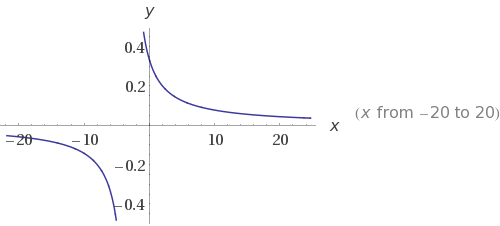
\includegraphics[width=0.7\textwidth]{plot1b.png}
\end{figure}

By intuition, we can see that it's not possible to fill in a $-3$ or $3$ as $x$, because that would lead to a division by zero which is an invalid operation.\\


$f(3) = \frac{3 - 3}{3^2 - 9} = \frac{3 - 3}{9 - 9} = \frac{0}{0}= $ not defined\\

$f(-3) = \frac{-3 - 3}{(-3)^2 - 9} = \frac{-6}{9 - 9} = \frac{-6}{0}= $ not defined\\

Domain:\\

$D(f) = \{ x \in \mathbb{R}: x \neq -3 \; and \; x \neq 3 \}$\\
  
Range:\\

$R(f) = \{ y \in \mathbb{R}: y \neq 0 \; and \; y \neq \frac{1}{6}\}$\\


\item[(c)] $f(x) = \frac{1}{\sqrt{x^2 - (3x + 4)}}$

\textbf{Solution:}\\

$f(x) = \frac{1}{\sqrt{x^2 - (3x + 4)}} = \frac{1}{\sqrt{x^2 - 3x - 4)}} =  \frac{1}{\sqrt{(x - 4)(x + 1)}}$\\

$f(0) = \frac{1}{\sqrt{0 - 0 - 4}} = \frac{1}{\sqrt{-4}} = $ not defined\\

$f(-1) = \frac{1}{\sqrt{1 + 3 - 4)}} = \frac{1}{\sqrt{0}} = \frac{1}{0} = $ not defined\\

$f(-2) = \frac{1}{\sqrt{4 + 6 - 4}} = \frac{1}{\sqrt{6}}$\\

$f(4) = \frac{1}{\sqrt{16 - 12 - 4}} = \frac{1}{\sqrt{0}} = \frac{1}{0} = $ not defined\\

$f(5) = \frac{1}{\sqrt{25 - 15 - 4}} = \frac{1}{\sqrt{6}}$\\

Domain:\\

$D(f) = \{ x \in \mathbb{R}: x < -1 \; or \; x > 4 \}$\\
  
Range:\\

$R(f) = \{ y \in \mathbb{R}: y > 0\}$\\


\end{itemize}







\item (\textbf{30 points}) After determining the domain and the range of the following functions, decide whether they are injective and/or surjective? Find the inverse of them if possible. If not possible, restrict the domain to make it possible.


\begin{itemize}


	\item[(a)] $f(x) = x^2 + 1$\\

	\textbf{Solution:}\\

Domain:\\

$D(f) = \{ x \in \mathbb{R} \}$\\

Range:\\

$R(f) = \{ y \in \mathbb{R}: y \geq 1\}$\\

Inverse: $f^{-1}(x) = \sqrt{x - 1}$ or $- \sqrt{x - 1} \; if \; x \geq 1$ \\

Injectivity: no\\
Surjectivity: no\\



	\item[(b)] $f(x) = ln(x - 1)$\\
	
	\textbf{Solution:}\\
	
$ln(x)$ is only defined for $x > 1$!\\
	
	
	
Domain:\\

$D(f) = \{ x \in \mathbb{R}: x > 1 \}$\\

Range:\\

$R(f) = \{ y \in \mathbb{R}\}$\\	
	
Inverse: $f^{-1}(x) = e^x + 1 \; if \; x > 1$\\	
	
Injectivity: no\\
Surjectivity: Surjective onto $\mathbb{R}$\\
	
	
	
	
	
	\item[(c)] $f(x) = \sqrt[3]{4 - x^3}$\\
	
	\textbf{Solution:}\\


Domain:\\

$D(f) = \{ x \in \mathbb{R}: x \leq 2^\frac{2}{3} \}$\\

Range:\\

$R(f) = \{ y \in \mathbb{R}: y \geq 0\}$\\	
	
Inverse: $f^{-1}(x) = \sqrt[3]{4 - x^3}$\\	
	
Injectivity: Injective on its domain\\	
Surjectivity: no\\

\end{itemize}


\item (\textbf{26 points}) Given the equation $5x - 4y = 9$


\begin{itemize}

	\item[(a)] Find the slope of the line having the equation above.\\
	
	\textbf{Solution:}\\
	
A common form of a linear equation in two variables x and y is 

\begin{equation}
	y = mx + b \notag
\end{equation}

where $m$ and $b$ designate constans. The constant $m$ determines the slope or gradient of that line and the constant term $b$ determines the point at which the line crosses the y-axis.\\		
	
So, we get the following:	
	
\begin{align}
5x - 4y  &= 9  \notag \\
-4y &= 9 - 5x \notag \\
y &= \frac{5}{4}x - \frac{9}{4} \notag
\end{align}
	
Answer; The slope of the equation $5x - 4y = 9$ is  $\frac{5}{4}$\\

	
	\item[(b)] Do the points $(1,-1)$, $(0, \pi$) and $(4,-2)$ lie on the line?\\
	
	\textbf{Solution:}\\
	
By filling in the x- and y-coordinates into the function from 3a) ($y = \frac{5}{4}x - \frac{9}{4}$), we can check, if the points lie on the line.\\

\begin{itemize}
	\item Point: (1,-1)
	
	\begin{align*}
		-1 &= \frac{5}{4}1 - \frac{9}{4} \notag \\
		-1 &= -\frac{4}{4} \notag \\
		-1 &= -1
	\end{align*}
	
Answer: Point (1, -1) lies on the line!\\

	\item Point: (0,$\pi$)
	
		\begin{align*}
		\pi &= \frac{5}{4}0 - \frac{9}{4} \notag \\
		\pi &= -\frac{9}{4} \notag \\
		\pi &= -\frac{9}{4}
	\end{align*}	
	
Answer: $\pi \neq -\frac{9}{4}$. Point (0, $\pi$) does not lie on the line!\\	


	\item Point: (4,-2)
	
			\begin{align*}
		-2 &= \frac{5}{4}4 - \frac{9}{4}\notag \\
		-2 &= \frac{20}{4} - \frac{9}{4} \\
		-2 &= \frac{11}{4}
	\end{align*}	
	
Answer: $-2 \neq \frac{11}{4}$. Point (4, -2) does not lie on the line!\\		
	
\end{itemize}



	
	
	\item[(c)] What is the distance between the origin and the point on the line of which x-coordinate is 13?\\
	
	\textbf{Solution:}\\

The origin on a graph is the point (0,0). First, we have to determine the y-coordinate of the point of which x-coordinate is 13:\\

\begin{align*}
	y &= \frac{5}{4}13 - \frac{9}{4} \notag \\
	y &= \frac{65}{4} - \frac{9}{4} \notag \\
	y &= \frac{56}{4} \notag \\
	y &= 14 \notag
\end{align*}

Therefore, the point is (13,14).\\

By applying the Pythagorean Theorem, we are able to determine the distance (let it be the hypotenuse "c" in the graphic) from point (13,14) to point (0,0) (the origin).\\

\begin{figure}[ht]
	\centering
  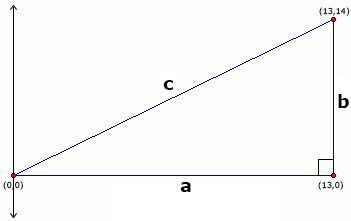
\includegraphics[width=0.6\textwidth]{pythagoras.jpg}
\end{figure}

Pythagorean Theorem: $a^2 + b^2 = c^2$\\

In this situation, a is 13 and b is 14. Therefore:\\

\begin{align*}
	c^2 &= 13^2 + 14^2 \notag \\
	c^2 &=  365 \notag \\
	c &= \sqrt{365} \notag	
		c \approx 19.105
\end{align*}

Answer: The distance between the origin and the point on the line of which x-coordinate is 13, is $\sqrt{365} \approx 19.105$

\end{itemize}


\item (\textbf{20 points}) Find the limits. (Hint: try to simplify as much as possible before applying the limit!)


\begin{itemize}

	\item[(a)] $\lim_{x \to 4} \frac{x - 4}{x^2 - 2x - 8}$\\
	
	\textbf{Solution:}\\
	
	$\lim_{x \to 4} \frac{x - 4}{x^2 - 2x - 8} = \lim_{x \to 4} \frac{x - 4}{(x+2)(x-4)}$\\
	
	Cancel out the common term in numerator and denominator, namely $(x-4)$, gives us:\\
	
	$\lim_{x \to 4} \frac{1}{(x+2)} = \frac{1}{6}$\\	
	
	Answer: $\lim_{x \to 4} \frac{x - 4}{x^2 - 2x - 8} = \frac{1}{6}$\\
	
	\item[(b)] $\lim_{x \to 3} \frac{x^3 - 27}{x^2 -9}$\\
	(Remember the identity $a^3 - b^3 = (a - b)(a^2 + ab + b^2)$)	
	
	\textbf{Solution:}\\
	
	$\lim_{x \to 3} \frac{x^3 - 27}{x^2 -9} = \lim_{x \to 3} \frac{x^3 - 3^3}{x^2 -3^2} = \lim_{x \to 3} \frac{(x-3)(x^2 + 3x + 9)}{(x-3)(x+3)}$\\
	
Cancel out the common term in numerator and denominator, namely $(x-3)$, gives us:\\	

$\lim_{x \to 3} \frac{(x^2 + 3x + 9)}{(x+3)} = \frac{27}{6} = \frac{9}{2}$\\

Answer: $\lim_{x \to 3} \frac{x^3 - 27}{x^2 -9} = \frac{9}{2}$\\
	
	\item[(c)] $\lim_{x \to h} \frac{2(x + h) - 2x}{h}$\\
	
	\textbf{Solution:}\\
	
	$\lim_{x \to h} \frac{2(x + h) - 2x}{h} = \lim_{x \to h} \frac{2x + 2h - 2x}{h} = \lim_{x \to h} \frac{2h}{h}$\\
	
	Cancel out the common term in numerator and denominator, namely $h$, gives us:\\
	
	$\lim_{x \to h} 2 = 2$\\
	
	The limit of a constant is the constant!\\
	
Answer: $\lim_{x \to h} \frac{2(x + h) - 2x}{h} = 2$\\	
	
	\item[(d)] $\lim_{x \to h} \frac{(x + h)^2 - x^2}{h}$\\

	\textbf{Solution:}\\
	
	By applying the first binomial formula $((a+b)^2 = a^2 + 2ab + b^2)$, it is possible to simplify the term.\\
	
		$\lim_{x \to h} \frac{(x + h)^2 - x^2}{h} = \lim_{x \to h} \frac{(h^2 + 2hx + x^2) - x^2}{h} = \lim_{x \to h} \frac{h^2 + 2hx}{h} = \lim_{x \to h} \frac{h(h + 2x)}{h}$\\

Cancel out the common term in numerator and denominator, namely $h$, gives us:\\

$\lim_{x \to h} h + 2x = 3h$\\
	

Answer: $\lim_{x \to h} \frac{(x + h)^2 - x^2}{h} = 3h$\\	

\end{itemize}


\end{enumerate}

\end{document}
